%% 
%% ACS project dissertation template. 
%% 
%% Currently designed for printing two-sided, but if you prefer to 
%% print single-sided just remove ",twoside,openright" from the 
%% \documentclass[] line below. 
%%
%%
%%   SMH, May 2010. 


\documentclass[a4paper,12pt,twoside,openright]{report}


%%
%% EDIT THE BELOW TO CUSTOMIZE
%%

\def\authorname{Jake Hillion\xspace}
\def\authorcollege{Queens' College\xspace}
\def\authoremail{Jake.Hillion@cl.cam.ac.uk}
\def\dissertationtitle{Void Processes: minimising privilege by default}
\def\wordcount{5}

\usepackage{courier}
\usepackage{dirtytalk} %quotations
\usepackage{epsfig}
\usepackage{graphicx}
\usepackage{listings}
\usepackage{multirow}
\usepackage[square,numbers]{natbib}
\usepackage{parskip}
\usepackage{setspace}
\usepackage{tabularx}
\usepackage[hidelinks]{hyperref}
\usepackage{verbatim}
\usepackage{xspace}

% TODO: remove me
\usepackage{todonotes}
\setuptodonotes{inline}

\setcounter{tocdepth}{1} % stop toc at sections

%% START OF DOCUMENT
\begin{document}
%TC:ignore

%% FRONTMATTER (TITLE PAGE, DECLARATION, ABSTRACT, ETC) 
\pagestyle{empty}
\singlespacing
% title page information
\begin{titlepage} 

\begin{center}
\noindent
\huge
\dissertationtitle \\
\vspace*{\stretch{1}}
\end{center}

\begin{center}
\noindent
\huge
\authorname \\
\Large
\authorcollege      \\[24pt]
%\begin{figure}

\includegraphics{CUni3.pdf}
%\end{figure}
\end{center}

\vspace{24pt} 

\begin{center}
\noindent
\large
{\it A dissertation submitted to the University of Cambridge \\ 
in partial fulfilment of the requirements for Part III of the
Computer Science Tripos.} 
\vspace*{\stretch{1}}
\end{center}

\begin{center}
\noindent
University of Cambridge \\
Computer Laboratory     \\
William Gates Building  \\
15 JJ Thomson Avenue    \\
Cambridge CB3 0FD       \\
{\sc United Kingdom}    \\
\end{center}

\begin{center}
\noindent
Email: \authoremail \\
\end{center}

\begin{center}
\noindent
\today
\end{center}

\end{titlepage} 

\newpage
\vspace*{\fill}

\onehalfspacing
\newpage
{\Huge \bf Declaration}

\vspace{24pt}

I, \authorname of \authorcollege, being a candidate for Computer
Science Tripos, Part III, hereby declare that this report and the
work described in it are my own work, unaided except as may be
specified below, and that the report does not contain material that
has already been used to any substantial extent for a comparable
purpose.

\vspace{24pt}
Total word count: \wordcount

\vspace{60pt}
\textbf{Signed}: 

\vspace{12pt}
\textbf{Date}: \today


\vfill

This dissertation is copyright \copyright 2022 \authorname. 
\\
All trademarks used in this dissertation are hereby acknowledged.



\newpage
\vspace*{\fill}

\singlespacing
\newpage
{\Huge \bf Abstract}
\vspace{24pt} 


Write a summary of the whole thing. Make 
sure it fits in one page. 


\newpage
\vspace*{\fill}


\pagenumbering{roman}
\setcounter{page}{0}
\pagestyle{plain}
\tableofcontents

%\listoffigures
%\listoftables

\onehalfspacing
\setstretch{1.2}

%TC:endignore
%% START OF MAIN TEXT

\chapter{Introduction}
\label{chap:introduction}

\pagenumbering{arabic} 
\setcounter{page}{1}

Void Processes allow running purpose-built applications without all of the features that a full Linux system makes available, and encourage privilege separation by default. This is achieved using a mixture of Linux namespaces and file descriptor based capabilities. During the process of building the system gaps in the kernel were exposed - namespaces were intended to emulate an ordinary Linux system rather than build something new. This work will go on to detail the mechanisms for creating Void Processes themselves, re-adding features that these processes need to do useful work, and describe which features are missing in the user-space kernel APIs to successfully create processes this way.

The question of what makes an operating system has been asked many times. There have previously been many attempts to redefine an operating system. Here we compare this work with two of those: unikernels and containers. Unikernels abandon the monolithic kernel in favour of a slimmed down kernel that only provides the features the user needs, limiting the trusted computing base but requiring special purpose applications to be written. Containers provide a view of an isolated system while sharing a monolithic kernel with the host, allowing almost any application that can run on Linux to run in a Linux Container, but including all of the features and security holes that come with running a monolithic kernel. Void Processes lie between the two. While they still rely on the monolithic kernel for isolation and inter-process communication, further reliance on the kernel is limited as much as possible. While much of the Linux experience is made unavailable the core calls remain the same, such as operations on file descriptors. By having nothing available at all by default, an environment where every privilege required must be explicitly added is created. When combined with inter-process communication, a feature not as ingrained in unikernels, high levels of privilege separation are achieved. These methods are plotted in Figure \ref{fig:least-to-most-linux}.

\begin{figure}[h]
    \centering
    
\includegraphics[width=0.6\textwidth]{figures/least-most-linux.png}
    \caption{Privilege separated environments plotted from least to most like bare metal Linux.}
    \label{fig:least-to-most-linux}
\end{figure}


\begin{table}
    \caption{Table showing the date and kernel version each namespace was added. The date provides the date of the first commit where they appeared, and the kernel version the kernel release they appear in the changelog of. Namespaces are ordered by kernel version then alphabetically. Some examples are provided of CVEs of each namespace, and CVEs that each namespace protects against.}

    \begin{center}
    \begin{tabular}{l|lr|lr|l|l}
        ns & \multicolumn{2}{l}{date} & \multicolumn{2}{|l|}{kernel ver.} & ns CVEs & prot. CVEs \\ \hline

        \texttt{mount}
            & Feb 2001 & \citep{viro_patchcft_2001}
            & 2.5.2 & \citep{torvalds_linux_2002}
            & 2020-29373
            & test \newline test2 \\

        \texttt{ipc}
            & Oct 2006 & \citep{korotaev_patch_2006}
            & 2.6.19 & \citep{linux_kernel_newbies_editors_linux_2006}
            &
            & \\

        \texttt{uts}
            & Oct 2006 & \citep{hallyn_patch_2006}
            & 2.6.19 & \citep{linux_kernel_newbies_editors_linux_2006}
            &
            & \\

        \texttt{user}
            & Jul 2007 & \citep{le_goater_user_2007}
            & 2.6.23 & \citep{linux_kernel_newbies_editors_linux_2007}
            & 2021-21284
            & \\

        \texttt{network}
            & Oct 2007 & \citep{biederman_net_2007}
            & 2.6.24 & \citep{linux_kernel_newbies_editors_linux_2008}
            & 2011-2189
            & \\

        \texttt{pid}
            & Oct 2006 & \citep{bhattiprolu_patch_2006}
            & 2.6.24 & \citep{linux_kernel_newbies_editors_linux_2008}
            & 2019-20794
            & \\

        \texttt{cgroup}
            & Mar 2016 & \citep{heo_git_2016}
            & 4.6 & \citep{torvalds_linux_2016}
            & 2022-0492
            & \\

        \texttt{time}
            & Nov 2019 & \citep{vagin_ns_2020}
            & 5.6 & \citep{linux_kernel_newbies_editors_linux_2020}
            &
            &

    \end{tabular}
    \end{center}

    \label{tab:namespaces}
\end{table}


\chapter{Privilege Separation}
\label{chap:priv-sep}

Many attack vectors exist in software, notably in argument processing and deserialisation \citep{the_mitre_corporation_improper_2006,the_mitre_corporation_deserialization_2006}. Creating security conscious applications requires one of two things: creating applications without security bugs, or separating the parts of the application with the potential to cause damage from the parts most likely to contain bugs. Though many efforts have been made to create correct applications [CN], the use of such technology is far from widespread and security related bugs in applications are still frequent [CN]. Rather than attempting to avoid bugs, the commonly employed solution is privilege separation: ensuring that the privileged portion of the application is separated from the portion which is likely to be attacked, and that the interface between them is correct. This chapter details what privilege separation is, why it is useful, and a summary of some of the privilege separation techniques available in modern Unices. Many of these techniques are included in some form in the final design for Void Processes.

\section{Privilege separation by process}

The basic unit of privilege separation on Unix is a process. If it's possible for an attacker to gain remote code execution in a process, the attacker gains access to all of that process's privilege. Reducing the privilege of a process therefore reduces the benefit of attacking that process. One solution to reducing privilege in the process is to take a previously monolithic application and split it into multiple smaller processes. Consider a TLS supporting web server that must have access to the certificate's private keys and also process user requests. These elements can be split into different processes. This means that if the user data handling process is compromised the attacker cannot access the contents of the private keys.

Application design in this paradigm is similar to that of a distributed system, where multiple asynchronous systems must interact over various communication channels. As an application becomes more like a networked system, serialisation and deserialisation becomes a common occurrence. As deserialisation is a very common source of exploits \citep{the_mitre_corporation_deserialization_2006}, this adds the potential for new flaws in the application.

OpenBSD is a UNIX operating system with an emphasis on security. A recent bug in OpenBSD's \texttt{sshd} highlights the utility of privilege separation \citep{the_openbsd_foundation_openssh_2022}. An integer overflow in the pre-authentication logic of the SSH daemon allowed a motivated attacker to exploit incorrect logic paths and gain access without authentication. Privilege separation ensures that the process with this bug, the pre-authentication process, is separated from the process which is able to be exploited, the highly privileged daemon. Moreover, privilege separation being mandatory in the software ensures that bugs which are not exploitable due to the privilege separation monitor's checks are not exploitable anywhere.

In 2003, privilege separation was added to the \texttt{syslogd} daemon of OpenBSD \citep{madhavapeddy_privsepc_2003}. The system is designed with a parent process that retains privilege and a network accepting child process that goes through a series of states, dropping privilege with each state change. This pattern allowed for restarting of the service while keeping the section which processed user data strongly separated from the process which remains privileged, by enabling the child process to cause its own restart while not holding enough privilege to execute that restart itself. An overview of the data flow is provided in Figure \ref{fig:openbsd-syslogd-privsep}.

\begin{figure}
    \centering
    
\includegraphics[width=0.4\textwidth]{figures/openbsd-syslogd-privsep.png}
    \caption{Data flow with the two processes in OpenBSD's privilege separated syslogd design.}
    \label{fig:openbsd-syslogd-privsep}
\end{figure}

\section{Privilege separation by time}

Many applications can privilege separate by using a single process which reduces its level of privilege as the application makes progress. This is effectively privilege separation over time. The approach is commonly to begin with high privilege for opening, for example, a listening socket below port 1000. After this has been completed, the ability to do so is dropped. One of the simplest ways to do this is to change user using \texttt{setuid(2)} after the privileged requirements are complete. An API such as OpenBSD's \texttt{pledge(2)} allows only a pre-specified set of system calls after the call to \texttt{pledge(2)}. A final alternative is to drop explicit capabilities on Linux. Each of these solutions irreversibly reduce the privilege of the process. This is known as dropping privilege. As the privilege has been irreversibly dropped, any attacker who gains control after the privilege has been dropped cannot take advantage of it.

After dropping privilege, it becomes difficult to do things such as reloading the configuration. The application process no longer has the required privilege to restart the application, and if it could gain it back then dropping it would have had no effect. This avoids having to treat the application as a distributed system as there continues to be only a single process to manage, which is often an easier paradigm to work in. The difficulty in implementing privilege dropping is ensuring that you know what privilege you hold, and drop it as soon as it is no longer required.

\section{Privilege separation by ownership}

The previous methods shown each suffer from knowing what their initial privilege is. An alternative method to enable the principle of least privilege in applications are object capabilities. An object capability is an unforgeable token of authority to perform some particular set of actions on some particular object.

While the methods looked at until now of privilege separation by process and time are supported by all Unices, object capabilities are a more niche system. Capsicum added object capabilities and was included in FreeBSD 10, released in January 2014 \citep{watson_capsicum_2010}. These capabilities may be shared between processes as with file descriptors. Capability mode removes access to all global namespaces from a process, allowing only operations on capabilities to continue. These capabilities are commonly those opened before the switch to capability mode, but they can also be sent and received (as file descriptors) or converted from a capability with more privilege to a capability with less.

Although object capabilities still require some additional work to ensure that only intentional capabilities remain accessible when entering capability mode, they come a lot closer to easy deprivileging than the previous solutions. However, their adoption remains limited at this point. They are unavailable in the latest Linux kernel release (5.17.7) at the time of writing, and there are no plans for their adoption.

\section{Privilege separation by perspective}

Linux approaches increased process separation using namespaces. Namespaces control the view of the world that a process sees. Processes remain the primary method of separation, but utilise namespaces to increase the separation between them. The intended and most common use case of namespaces is providing containers. Containers approximate virtual machines, providing the appearance of running on an isolated system while sharing the same host. Containers, however, have to implement privilege separation in a very different way to the privilege separation we've seen previously. Rather than spawning multiple processes and employing privilege separation techniques to limit the attack vector in each, one spawns multiple containers to form a more literal distributed system. It is common to see, for example, a web server and the database that backs it deployed as two separate containers. These separate containers interact entirely over the network. This means that if a user achieves remote code execution of the database, it does not extend to the web server. This presents an interesting paradigm of small applications which can and often do run on separate physical hosts combining to provide a unified application experience.

\section{Summary}

This work focuses on the application of namespaces to more conventional privilege separation. Working with a shim which orchestrates the process and namespace layout, Void Applications seek to provide a completely pruned minimal Linux experience to each Void Process within the application. This builds on much of the prior work to severely limit the access of processes in the application. There is never a need to drop privileges as processes are created with the absolute minimum privilege necessary to perform correctly. In Chapter \ref{chap:entering-the-void} we discuss each namespace's role in Linux and how to create one which is empty, before explaining in Chapter \ref{chap:filling-the-void} how to reinsert just enough Linux for each process in an application to be able to complete useful work. These combine to form an architecture which minimises privilege by default, motivating highly intentional privilege separation.


\chapter{Entering the Void}
\label{chap:entering-the-void}

Isolating parts of a Linux system from the view of certain processes is achieved using namespaces. Namespaces are commonly used to provide isolation in the context of containers, which provide the appearance of an isolated Linux system to contained processes. Instead, with Void Processes, we use namespaces to provide a view of a system that is as minimal as possible, while still sitting atop the Linux kernel. In this chapter each namespace available in Linux 5.15 LTS is discussed. The objects each namespace protects are presented and security vulnerabilities discussed. Then the method for entering a void with each namespace is given along with a discussion of the difficulties associated with this in current Linux. Chapter \ref{chap:filling-the-void} goes on to explain how necessary features for applications are added back in.

The full set of namespaces are represented in Table \ref{tab:namespaces}, in chronological order. The chronology of these is important in understanding the thought process behind some of the design decisions. The ease of creating an empty namespace varies massively, as although adding namespaces shared the goal of containerisation, they were completed by many different teams of people over a number of years. Some namespaces maintain strong connections to their parent, while others are created with absolute separation. We start with those that are most trivial to add, working up to the namespaces most intensely linked to their parents.

\section{ipc namespaces}
\label{sec:voiding-ipc}

IPC namespaces isolate two mechanisms that Linux provides for IPC which aren't controlled by the filesystem. System V IPC and POSIX message queues are each accessed in a global namespace of keys. This has created issues in the past with attempting to run multiple instances of PostgreSQL on a single machine, as both instances use System V IPC objects which collide \citep[§4.3]{barham_xen_2003}. IPC namespaces solve this effectively for containers by creating a new scoped namespace. Processes are a member of one and only one IPC namespace, allowing the familiar global key APIs.

IPC namespaces are optimal for creating Void Processes. From the manual page \citep{free_software_foundation_ipc_namespaces7_2021}:

\say{Objects created in an IPC namespace are visible to all other processes that are members of that namespace, but are not visible to  processes  in  other  IPC  namespaces.}

This provides exactly the correct semantics for a Void Process. IPC objects are visible within a namespace if and only if they are created within that namespace. Therefore, a new namespace is entirely empty, and no more work need be done.

\todo{Add vulnerabilities protected from. Discuss lack of vulnerabilities relating to the namespace itself.}

\section{uts namespaces}
\label{sec:voiding-uts}

UTS namespaces provide isolation of the hostname and domain name of a system between processes. Similarly to IPC namespaces, all processes in the same namespace see the same results for each of these values. This is useful when creating containers. If unable to hide the hostname, each container would look like the same machine. Unlike IPC namespaces, UTS namespaces are inherit their values. Each of the hostname and domain name in the new namespace is initialised to the values of the parent namespace.

As the inherited value does give information about the world outside of the Void Process, slightly more must be done than placing the process in a new namespace. Fortunately this is easy for UTS namespaces, as the host name and domain name can be set to constants, removing any link to the parent. Although the implementation of this is trivial, it highlights how easy the information passing elements of each namespace are to miss if manually implementing isolation with namespaces.

\todo{Add vulnerabilities protected from. Discuss lack of vulnerabilities relating to the namespace itself.}

\section{time namespaces}
\label{sec:voiding-time}

Time namespaces are the final namespace added at the time of writing, added in kernel version 5.6 \citep{linux_kernel_newbies_editors_linux_2020}. The motivation for adding time namespaces is given in the manual page \citep{free_software_foundation_time_namespaces7_2021}:

\say{The  motivation  for adding time namespaces was to allow the monotonic and boot-time clocks to maintain consistent values during container migration and checkpoint/restore.}

That is, time namespaces virtualise the appearance of system uptime to processes. They do not attempt to virtualise wall clock time. This is important for processes that depend on time in primarily one situation: migration. If an uptime dependent process is migrated from a machine that has been up for a week to a machine that was booted a minute ago, the guarantees provided by the clocks \texttt{CLOCK\_MONOTONIC} and \texttt{CLOCK\_BOOTTIME} no longer hold. This results in time namespaces having very limited usefulness in a system that does not support migration, such as the one presented here. Perhaps randomised offsets would hide some information about the system, but the usefulness is limited. Time namespaces are thus avoided in this implementation.

Searching the list of released CVEs for both "clock`` and "time linux`` (time itself revealed significantly too many results to parse) shows no vulnerabilities in the time subsystem on Linux, or the time namespaces themselves. This supports not including time namespaces at this stage, as their range is very limited, particularly in terms of isolation from vulnerabilities.

\section{network namespaces}
\label{sec:voiding-net}

Network namespaces on Linux isolate the system resources related to networking. These include network interfaces themselves, IP routing tables, firewall rules and the \texttt{/proc/net} directory. This level of isolation allows a network stack that operates completely independently to exist on a single kernel.

Similarly to IPC, network namespaces present the optimal namespace for running a Void Process. Creating a new network namespace immediately creates a namespace containing only a local loopback adapter. This means that the new network namespace has no link whatsoever to the creating network namespace, only supporting internal communication. To add a link, one can create a virtual Ethernet pair with one adapter in each namespace (Figure \ref{fig:virtual-ethernet}). Alternatively, one can create a Wireguard adapter with sending and receiving sockets in one namespace and the VPN adapter in another \citep[§7.3]{donenfeld_wireguard_2017}. These methods allow for very high levels of separation while still maintaining access to the primary resource - the Internet or wider network. Further, this design places the management of how connected a namespace is to the parent in user-space. This is a significant difference compared to some of the namespaces discussed later in this chapter.

\begin{figure}
\begin{minipage}{.45\textwidth}

\lstset{caption={}}
\begin{lstlisting}[frame=tlrb,showlines=true]{Name}
#
#
# ip link add veth0 type veth peer veth1
# ip link set veth1 netns test
# ip addr add 192.168.0.1/24 dev veth0
# ip link set up dev veth0
# ping -c 1 192.168.0.2
PING 192.168.0.2 (192.168.0.2) 56(84) bytes of data.
64 bytes from 192.168.0.2: icmp_seq=1 ttl=64 time=0.317 ms
\end{lstlisting}

\end{minipage}\hfill
\begin{minipage}{.45\textwidth}

\lstset{caption={}}
\begin{lstlisting}[frame=tlrb]{Name}
# unshare -n
# ip netns attach test $$
#
#
# ip addr add 192.168.0.2/24 dev veth1
# ip link set up dev veth1
# ping -c 1 192.168.0.1
PING 192.168.0.1 (192.168.0.1) 56(84) bytes of data.
64 bytes from 192.168.0.1: icmp_seq=1 ttl=64 time=0.107 ms
\end{lstlisting}

\end{minipage}

\caption{Creating a virtual Ethernet pair between the root network namespace and a newly created network namespace.}
\label{fig:virtual-ethernet}
\end{figure}

Network namespaces are also the first mentioned to control access to \texttt{procfs}. \texttt{/proc} holds a pseudo-filesystem which controls access to many of the kernel data structures that aren't accessed by system calls. Seeing the intended behaviour here requires remounting \texttt{/proc}, which must be done with extreme care so as not to overwrite it for every other process. In a Void Process this is handled by automatically voiding the mount namespace, meaning that this does not need to be intentionally taken care of.

\todo{Add vulnerabilities protected from. Discuss lack of vulnerabilities relating to the namespace itself.}

\section{pid namespaces}
\label{sec:voiding-pid}

PID namespaces create a mapping from the process IDs inside the namespace to process IDs in the parent namespace. This continues until processes reach the top-level, named init, PID namespace. This isolation behaviour is different to that of the namespaces discussed thus far, as each process within the namespace represents a process in the parent namespace too, albeit with different identifiers.

As with network namespaces, PID namespaces have a significant effect on \texttt{/proc}. Further, they cause some unusual behaviour regarding the PID 1 (init) process in the new namespace. These behaviours are shown in Listing \ref{lst:unshare-pid}. The first behaviour shown is that an \texttt{unshare(CLONE\_PID)} call followed immediately by an \texttt{exec} does not create a working shell. The reason for this is that the first process created in the new namespace is given PID 1 and acts as an init process. That is, whichever process the shell spawns first becomes the init process of the namespace, and when that process dies, the namespace can no longer create new processes. This behaviour is avoided by either calling \texttt{unshare(2)} followed by \texttt{fork(2)}, or utilising \texttt{clone(2)} instead, both of which ensure that the correct process is created first in the new namespace. The \texttt{unshare(1)} binary provides a fork flag to solve this, while the implementation of the Void Orchestrator uses \texttt{clone(2)} which has the semantics of combining the two into a single syscall.

Secondly, we see that even in a shell that appears to be working correctly, processes from outside of the new PID namespace are still visible. This behaviour occurs because the mount of \texttt{/proc} visible to the process in the new PID namespace is the same as the init process. This is solved by remounting \texttt{/proc}, available to \texttt{unshare(3)} with the \texttt{---mount-proc} flag. Care must be taken that this mount is completed in a new mount namespace, or else processes outside of the PID namespace will be affected. The Void Orchestrator again avoids this by voiding the mount namespace entirely, meaning that any access to \texttt{procfs} must be either freshly mounted or bound to outside the namespace intentionally.

\lstset{caption={Unshare behaviour with PID namespaces, with and without forking and remounting proc.}}
\begin{lstlisting}[float,label={lst:unshare-pid}]
$ unshare --pid
-bash: fork: Cannot allocate memory
# (new shell in new pid namespace)
# ps ax | tail -n 3
-bash: fork: Cannot allocate memory

$ unshare --fork --pid
# (new shell in new pid namespace)
# ps ax | tail -n 3
2645 ?        I      0:00 [kworker/...]
2689 pts/1    R+     0:00 ps ax
2690 pts/1    S+     0:00 tail -n 2

$ unshare --fork --mount-proc --pid
# (new shell in new pid namespace)
# ps ax | tail -n 3
 1 pts/1    S      0:00 -bash
15 pts/1    R+     0:00 ps ax
16 pts/1    S+     0:00 tail -n 3

\end{lstlisting}

\todo{Add vulnerabilities protected from. Discuss lack of vulnerabilities relating to the namespace itself.}

\section{mount namespaces}
\label{sec:voiding-mount}

Mount namespaces were by far the most challenging part of this project. When adding new features, they continuously raised problems in both API description, expected behaviour, and availability of tools in user-space. A comparison will be given in this section to two other namespaces, network and UTS, to show the significant differences in the design goals of mount namespaces. Many of the implementation problems here comes from a fundamental lack of consistency between mount namespaces and other namespaces in Linux.

\subsection{Copy-on-Write}

Comparing to network namespaces, we see a huge difference in what occurs when a new namespace is created. When creating a new network namespace, the ideal conditions for a Void Process are created - a network namespace containing only a loopback adapter. That is, the process has no ability to interact with the outside network, and no immediate relation to the parent network namespace. To interact with alternate namespaces, one must explicitly create a connection between the two, or move a physical adapter into the new (empty) namespace. Mount namespaces, rather than creating a new and empty namespace, made the choice to create a copy of the parent namespace, in a copy-on-write fashion. That is, after creating a new mount namespace, the mount hierarchy appears much the same as before. This is shown in Listing \ref{lst:unshare-cat-passwd}, where the file \texttt{/etc/passwd} is shown before and after an unshare, revealing the same content.

\lstset{caption={Reading the same file before and after unsharing the mount namespace.}}
\begin{lstlisting}[float,label={lst:unshare-cat-passwd}]
int main() {
int fd;

if ((fd = open("/etc/passwd", O_RDONLY)) < 0)
    perror("open");
print_file(fd);
if (close(fd))
    perror("close");

if (unshare(CLONE_NEWNS))
    perror("unshare");
printf("----- unshared -----\n");

if ((fd = open("/etc/passwd", O_RDONLY)) < 0)
    perror("open");
print_file(fd);
if (close(fd))
    perror("close");
}
--

root:x:0:0:root:/root:/bin/bash
daemon:x:1:1:daemon:/usr/sbin:/usr/sbin/nologin
bin:x:2:2:bin:/bin:/usr/sbin/nologin
sys:x:3:3:sys:/dev:/usr/sbin/nologin
...
----- unshared -----
root:x:0:0:root:/root:/bin/bash
daemon:x:1:1:daemon:/usr/sbin:/usr/sbin/nologin
bin:x:2:2:bin:/bin:/usr/sbin/nologin
sys:x:3:3:sys:/dev:/usr/sbin/nologin
...
\end{lstlisting}

\subsection{Shared Subtrees}

While some other namespaces are copy-on-write, for example UTS namespaces, they do not present the same problem as mount namespaces. Although UTS namespaces are copy-on-write, it is trivial to create the conditions for a Void Process by setting the hostname of the machine to a constant. This removes any relation to the parent namespace and to the outside machine. Mount namespaces instead maintain a shared pointer with most filesystems, more akin to not creating a new namespace than a copy-on-write namespace.

Shared subtrees \citep{pai_shared_2005} were introduced to provide a consistent view of the unified hierarchy between namespaces. Consider the example in Figure \ref{fig:shared-subtrees}. \texttt{unshare(1)} creates a non-shared tree, which presents the behaviour shown. Although \texttt{/mnt/cdrom} from the parent namespace has been bind mounted in the new namespace, the content of \texttt{/mnt/cdrom} is not the same. This is because the filesystem newly mounted on \texttt{/mnt/cdrom} is unavailable in the separate mount namespace. To combat this, shared subtrees were introduced. That is, as long as \texttt{/mnt/cdrom} resides on a shared subtree, the newly mounted filesystem will be available to a bind of \texttt{/mnt/cdrom} in another namespace. \texttt{systemd} made the choice to mount \texttt{/} as a shared subtree \citep{free_software_foundation_mount_namespaces7_2021}:

\begin{figure}
\begin{minipage}{.45\textwidth}

\lstset{caption={}}
\begin{lstlisting}[frame=tlrb,showlines=true]{Name}
# unshare -m
# mount_container_root /tmp/a
# mount --bind \
    /mnt/cdrom /tmp/a/mnt/cdrom
# pivot_root /tmp/a /tmp/a/oldroot
# umount /tmp/a/oldroot
#
# ls /mnt/cdrom

\end{lstlisting}

\end{minipage}\hfill
\begin{minipage}{.45\textwidth}

\lstset{caption={}}
\begin{lstlisting}[frame=tlrb]{Name}
#
#
#
#
#
#
# mount /dev/sr0 /mnt/cdrom
# ls /mnt/cdrom
file_1 file_2
\end{lstlisting}

\end{minipage}

\caption{Highly separated behaviour without shared subtrees between mount namespaces.}
\label{fig:shared-subtrees}
\end{figure}

\say{Notwithstanding the fact that the default propagation type for new mount is in many cases \texttt{MS\_PRIVATE}, \texttt{MS\_SHARED} is typically more useful.  For this reason, \texttt{systemd(1)} automatically remounts all mounts as \texttt{MS\_SHARED} on system startup. Thus, on most modern systems, the default propagation type is in practice \texttt{MS\_SHARED}.}

This means that when creating a new namespace, mounts and unmounts are propagated by default. More specifically, it means that mounts and unmounts are propagated both from the parent namespace to the child, and from the child namespace to the parent. This can be highly confusing behaviour, as it provides minimal isolation by default. \texttt{unshare(1)} considers this behaviour inconsistent with the goals of unsharing - it immediately calls \texttt{mount("none", "/", NULL, MS\_REC|MS\_PRIVATE, NULL)} after \texttt{unshare(CLONE\_NEWNS)}, detaching the newly unshared tree. The reasoning for enabling \texttt{MS\_SHARED} by default is that containers created should not present the behaviour given in Figure \ref{fig:shared-subtrees}, and this behaviour is unavoidable unless the parent mounts are shared, while it is possible to disable the behaviour where necessary.

\subsection{Lazy unmounting}

Mount namespaces present further interesting behaviour when unmounting the old root filesystem. Although this may initially seem isolated to Void Processes, it is also a problem in a container system. Consider again the container created in Figure \ref{fig:shared-subtrees}: the existing root must be unmounted after pivoting, else the container remains fully connected to the outside root.

Referring again to network namespaces, sockets continue to exist in their initial namespace, allowing for regular file-descriptor passing semantics \citep{biederman_re_2007}. Extending upon this socket behaviour is Wireguard, which creates adapters that may be freely moved between namespaces while continuing to connect externally from their initial parent \citep[§7.3]{donenfeld_wireguard_2017}.

Something which behaves differently is the memory mapping of a currently running process's binary. Consider the example in Listing \ref{lst:unshare-umount}, which shows a short C program and the result of running it. It is seen that the \texttt{/} mount is busy when attempting the unmount. Given that the process was created in the parent namespace, the behaviour of file descriptors would suggest that the process would maintain a link to the parent namespace for its own memory mapped regions. However, the fact that the otherwise empty namespace has a busy mount shows that this is not the case.

\lstset{caption={Behaviour when attempting to unmount / after an unshare.}}
\begin{lstlisting}[float,label={lst:unshare-umount}]
int main() {
if (unshare(CLONE_NEWNS))
	perror("unshare");
if (mount("none", "/", NULL,
  MS_REC|MS_PRIVATE, NULL))
	perror("mount");
if (umount("/"))
	perror("umount");
}
--
umount: Device or resource busy
\end{lstlisting}

A feature called lazy unmounting or \texttt{MNT\_DETACH} exists for situations where a busy mount still needs to be unmounted. Supplying the \texttt{MNT\_DETACH} flag to \texttt{umount2(2)} causes the mount to be immediately detached from the unified hierarchy, while remaining mounted internally until the last user has finished with it. Whilst this initially seems like a good solution, this syscall is incredibly dangerous when combined with shared subtrees. This behaviour is shown in Figure \ref{fig:unshare-umount-lazy}, where a lazy (and hence recursive) unmount is combined with a shared subtree to disastrous effect.

\begin{figure}
\begin{minipage}{.45\textwidth}

\lstset{caption={}}
\begin{lstlisting}[frame=tlrb,showlines=true]{Name}
# cat /proc/mounts | grep udev
udev /dev devtmpfs rw,nosuid,relati...
#
#
# cat /proc/mounts | grep udev
cat: /proc/mounts: No such file or...
\end{lstlisting}
\end{minipage}\hfill
\begin{minipage}{.45\textwidth}

\lstset{caption={}}
\begin{lstlisting}[frame=tlrb]{Name}
#
#
# unshare --propagation unchanged -m
# umount -l /
#
#
\end{lstlisting}

\end{minipage}

\caption{Behaviour when attempting to unmount / from an unshared shell with a shared mount.}
\label{fig:unshare-umount-lazy}
\end{figure}

This behaviour raises questions about why a shared subtree, which exists as an object, would need to be detached recursively - decreasing the reference count to the shared subtree itself would seem sufficient. The inconsistency is best explained by looking at the development timeline for the three features here: mount namespaces, shared subtrees, and recursive lazy unmounts. When lazy unmounting was added, in September 2001, the author said the following (sic) \citep{viro_patch_2001}:

\say{There are only two things to take care of -
	a) if we detach a parent we should do it for all children
	b) we should not mount anything on "floating" vfsmounts.
Both are obviously staisfied for current code (presence of children
means that vfsmount is busy and we can't mount on something that
doesn't exist).}

This logic held even in the presence of namespaces, with the initial patchset in February 2001 \citep{viro_patch_2001}, as mounts were not initially shared but duplicated between namespaces. However, when shared subtrees were added in January 2005 \citep{viro_rfc_2005}, this logic stopped holding.

When setting up a container environment, one calls \texttt{pivot\_root(2)} to replace the old root with a new root for the container. Then, the old root may be unmounted. Oftentimes the solution is to exec a binary in the new root first, meaning that the old root is no longer in use and may be unmounted. This works, as old root is only a reference in this namespace, and hence may be unmounted with children - the \texttt{vfsmount} in this namespace is not busy, contradicting an assertion in the quotation.

If, instead, one wishes to continue running the existing binary, this is possible with lazy unmounting. However, the kernel only exposes a recursive lazy unmount. With shared subtrees, this results in destroying the parent tree. While this is avoidable by removing the shared propagation from the subtree before unmounting, the choice to have \texttt{MNT\_DETACH} aggressively cross shared subtrees can be highly confusing, and perhaps undesired behaviour in a world with shared subtrees by default.

The API is particularly unfriendly to creating a Void Process. The creation of mount namespaces is copy-on-write, and many filesystems are mounted shared. This means that they propagate changes back through namespace boundaries. As the mount namespace does not allow for creating an entirely empty root, extra care must be taken in separating processes. The method taken in this system is mounting a new \texttt{tmpfs} file system in a new namespace, which doesn't propagate to the parent, and using the \texttt{pivot\_root(8)} command to make this the new root. By pivoting to the \texttt{tmpfs}, the old root exists as the only reference in the otherwise empty \texttt{tmpfs}. Finally, after ensuring the old root is set to \texttt{MNT\_PRIVATE} to avoid propagation, the old root can be lazily detached. This allows the binary from the parent namespace, the shim in this case, to continue running correctly. Any new processes only have access to the materials in the empty \texttt{tmpfs}. This new \texttt{tmpfs} never appears in the parent namespace, separating the Void Process effectively from the parent namespace.

\todo{Add vulnerabilities protected from. Discuss lack of vulnerabilities relating to the namespace itself.}

\section{user namespaces}
\label{sec:voiding-user}

User namespaces provide isolation of security between processes. They isolate uids, gids, the root directory, keys and capabilities. This provides massive utility for rootless containers [CN], and also this shim. Rather than the shim being a \texttt{setuid} or \texttt{CAP\_SYS\_ADMIN} binary, it can instead operate with ambient authority. This vastly simplifies the logic for opening file descriptors to pass the child processes, as the shim itself is already operating with correctly limited authority.

Similarly to many other namespaces, user namespaces suffer from needing to limit their isolation. For a user namespace to be useful, some relation needs to exist between processes in the user namespace and objects outside. That is, if a process in a user namespace shares a filesystem with a process in the parent namespace, there should be a way to share credentials. To achieve this with user namespaces a mapping between users in the namespace and users outside exists. The most common use-case is to map root in the user namespace to the creating user outside, meaning that a process with full privileges in the namespace will be constrained to the creating user's ambient authority.

To create an effective Void Process content must be written to the files \texttt{/proc/[pid]/uid\_map} and \texttt{/proc/[pid]/gid\_map}. In the case of the shim uid 0 and gid 0 are mapped to the creating user. This is done first such that the remaining stages in creating a Void Process can have root capabilities within the user namespace - this is not possible prior to writing to these files. Otherwise, \texttt{CLONE\_NEWUSER} combines effectively with other namespace flags, ensuring that the user namespace is created first. This enables the other namespaces to be created without additional permissions.

\todo{Discuss how intense the restrictions on who can do what are. Add vulnerabilities protected from. Discuss lack of vulnerabilities relating to the namespace itself.}

\section{cgroup namespaces}
\label{sec:voiding-cgroup}

cgroup namespaces provide limited isolation of the cgroup hierarchy between processes. Rather than showing the full cgroups hierarchy, they instead show only the part of the hierarchy that the process was in on creation of the new cgroup namespace. Correctly creating a Void Process is hence as follows:

\begin{enumerate}
    \item Create an empty cgroup leaf.
    \item Move the new process to that leaf.
    \item Unshare the cgroup namespace.
\end{enumerate}

This process excludes the cgroup namespace from the initial \texttt{clone(3)} call, as the cloned process must be moved before creating the new namespace. By following this sequence of calls, the process in the void can only see the leaf which contains itself and nothing else, limiting access to the host system.  This is the approach taken in this piece of work. Running the shim with ambient autrhoirty here presents an issue, as the cgroup hierarchy relies on discretionary access control. In order to move the process into a leaf the shim must have sufficient authority to modify the cgroup hierarchy. On systemd these processes will be launched underneath a user slice and will have sufficient permissions, but this may vary between systems. This leaves cgroups the most weakly implemented namespace at present.

Although good isolation of the host system from the Void Process is provided, the Void Process is in no way hidden from the host. There exists only one cgroups v2 hierarchy on a system (cgroups v1 are ignored for clarity), where resources are delegated through each. This means that all processes contained within the hierarchy must appear in the init hierarchy, such that the distribution of the single set of system resources can be centrally controlled. This behaviour is similar to the aforementioned pid namespaces, where each process has a distinct PID in each of its parents, but does show up in each.

There are two problems when working with cgroups namespaces in user-space: needing sufficient discretionary access control, and leaving the control of individual application processes in a global namespace. An alternative kernel design would increase the utility by solving both of these problems. A process in a new cgroups namespace could instead create a detached hierarchy with the process as a leaf of the root and full permissions in the user-namespace that created it. The main cgroups hierarchy could then still see a single application to control, while the application itself would have full access over sharing its resources.  This presents the ability for mechanisms of managing cgroups to clash between the namespaces, as the outer namespace would now have control over what resources are delegated to the application rather than each process in the application. Such a system would also provide improved behaviour over the current, which requires a delegation flag to be handed to the manager informing it to go no further down the tree. This would be significantly better enforced with namespaces. That is, the main namespace could be handled by \texttt{systemd}, while the \texttt{/docker} namespace could be internally managed by docker. This would allow \texttt{systemd} to move the \texttt{/docker} namespace around as required, with no awareness of the choices made internally.

\todo{Add vulnerabilities protected from. Discuss lack of vulnerabilities relating to the namespace itself.}

\section{Summary}

In this chapter I presented the 8 namespaces available in Linux 5.15. What each namespace protects against, how to completely empty each created namespace, and the constraints in doing so were presented. For cgroup and mount namespaces, alternative designs that increase the usability of the namespaces were discussed.

Now that the motivation for emptying namespaces has been shown with the avoidance of vulernabilities, facilities to re-expose some of the system must be introduced in order to make useful applications. The methods for reintroducing parts of the system are given in Chapter \ref{chap:filling-the-void}, before demonstrating how to build useful applications in Chapter \ref{chap:building-apps}.


\chapter{Filling the Void}
\label{chap:filling-the-void}

Now that a completely empty set of namespaces are available for a Void Process, the ability to reinsert specific privileges must be added to support non-trivial applications. To allow for running applications as Void Processes with minimal kernel changes, this is achieved using a mixture of file-descriptor capabilities and adding elements to the empty namespaces. Capabilities allow for very explicit privilege passing where suitable, while adding elements to namespaces supports more of Linux's modern features.

\section{mount namespace}
\label{sec:filling-mount}

There are two options to provide access to files and directories in the void. Firstly, for a single file, an opened file descriptor can be offered. Consider the TLS broker of a TLS server with a persistent certificate and keyfile. Only these files are required to correctly run the application - no view of a filesystem is necessary. Providing an already opened file descriptor gives the process a capability to those files while requiring no concept of a filesystem, allowing that to remain a complete void. This is possible because of the semantics of file descriptor passing across namespaces - the file descriptor remains a capability, regardless of moving into a namespace without access to the file in question.

Alternatively, files and directories can be mounted in the Void Process's namespace. This supports three things which the capabilities do not: directories, dynamic linking, and applications which have not been adapted to use file descriptors. Firstly, the existing \texttt{openat(2)} calls are not suitable by default to treat directory file descriptors as capabilities, as they allow the search path to be absolute. This means that a process with a directory file descriptor in another namespace can access any files in that namespace [RN] by supplying an absolute path. Secondly, dynamic linking is best served by binding files, as these read only copies and the trusted binaries ensure that only the required libraries can be linked against. Finally, support for individual required files can be added by using file descriptors, but many applications will not trivially support it. Binding files allows for some backwards compatibility with applications that are more difficult to adapt.

\section{network namespace}
\label{sec:filling-net}

Reintroducing networking to a Void Process follows a similar capability-based paradigm to reintroducing files. Rather than providing the full Linux networking subsystem to a Void Process, it is instead handed a file descriptor that already has the requisite networking permissions. A capability for an inbound networking socket can be requested statically in the application's specification, which fits well with the earlier specified threat model. This socket remains open and allows the application to continuously accept requests, generating the appropriate socket for each request within the application itself. These request capabilities can be dealt with in the same process or handed back to the shim to be distributed to another Void Process.

Outbound networking is more difficult to re-add to a Void Process than inbound networking. The approach that containerisation solutions such as Docker take by default is using NAT with bridged adapters [RN]. That is, the container is provided an internal IP address that allows access to all networks via the host. Virtual machine solutions take a similar approach, creating bridged Ethernet adapters on the outside network or on a private NAT. Each of these approaches give the container/machine the appearance of unbounded outbound access, relying on firewalls to limit this afterwards. This does not fit well with the ethos of creating a Void Process - minimum privilege by default. An ideal solution would provide precise network access to the void, rather than adding all access and restricting it in post. This is achieved with inbound sockets by providing the precise and already connected socket to an otherwise empty network namespace, which does not support creating exposed inbound sockets of its own.

Consideration is given to providing outbound access with statically created and passed sockets, the same as inbound access. For example, a socket to a database could be specified in the specification, or even one per worker process. The downside of this approach is that the socket lifecycle is still handled by the kernel. While this could work well with UDP sockets, TCP sockets can fail because the remote was closed or a break in the path caused a timeout to be hit.

Given that statically giving sockets is infeasible and adding a firewall does not fit well with creating a void, I sought an alternative API. \texttt{pledge(2)} is a system call from OpenBSD which restricts future system calls to an approved set \citep{the_openbsd_foundation_pledge2_2022}. This seems like a good fit, though operating outside of the operating system makes the implementation very different. Acceptable sockets are specified in the application specification, then an interaction socket is provided to request various pre-approved sockets from the shim layer. This allows limited access to the host network, approved or denied at request time instead of by a firewall. That is, access to a precisely configured socket can be injected to the void, with a capability to request such sockets and a capability given for each socket requested.

\section{user namespace}
\label{sec:filling-user}

Filling a user namespace is a slightly odd concept compared to the namespaces already discussed in this section. As stated in Section \ref{sec:voiding-user}, a user namespace comes with no implicit mapping of users whatsoever. To enable applications to be run with bounded authority, a single mapping is added by the Void Orchestrator of \texttt{root} in the child user namespace to the launching UID in the parent namespace. This means that the user with highest privilege in the container, \texttt{root}, will be limited to the access of the launching user. The behaviour of mapping \texttt{root} to the calling user is shown with the \texttt{unshare(1)} command in Listing \ref{lst:mapped-root-directory}, where a directory owned by the calling user, \texttt{jsh77}, appears to be owned by \texttt{root} in the new namespace. A file owned by \texttt{root} in the parent namespace appears to be owned by \texttt{nobody} in the child namespace, as no mapping exists for that file's user.

\lstset{language=C,caption={A directory listing before and after entering a user namespace with mapped root.}}
\begin{lstlisting}[float,label={lst:mapped-root-directory}]
$ ls -ld repos owned_by_root
-rw-r--r-- 1 root  root     0 May  7 22:13 owned_by_root
drwxrwxr-x 7 jsh77 jsh77 4096 Feb 27 17:52 repos

$ unshare -U --map-root

# ls -ld repos owned_by_root
-rw-r--r-- 1 nobody nogroup    0 May  7 22:13 owned_by_root
drwxrwxr-x 7 root root 4096 Feb 27 17:52 repos
\end{lstlisting}

The way user namespaces are currently used creates a binary system: either a file appears as owned by \texttt{root} if owned by the calling user, or appears as owned by \texttt{nobody} if not (ignoring groups for clarity, though their behaviour is similar). One questions whether more users could be mapped in, but this presents additional difficulties. Firstly, \texttt{setgroups(2)} system call must be denied to achieve correct behaviour in the child namespace. This is because the \texttt{root} user in the child namespace has full capabilities, which include \texttt{CAP\_SETGID}. This means that the user in the namespace can drop their groups, potentially allowing access to materials which the creating user did not (consider a file with permissions \texttt{0707}). This limits the utility of switching user in the child namespace, as the groups must remain the same. Secondly, mapping to users and groups other than oneself requires \texttt{CAP\_SETUID} or \texttt{CAP\_SETGID} in the parent namespace. Avoiding this is well advised to reduce the ambient authority of the shim.

Voiding the user namespace initially provides the ability to create other namespaces with ambient authority, and hides the details of the Void Process's ambient permissions from inside. Although this creates a binary system of users which may at first seem limiting, applying the context of Void Processes demonstrates that it is not. Linux itself may utilise users, groups and capabilities for process limits, but Void Processes only provide what is absolutely necessary. That is, if a process should not have access to a file owned by the same user, it is simply not made available. Running only as \texttt{root} within the Void Process is therefore not a problem - multiple users is a feature of Linux which doesn't assist Void Processes in providing minimum privilege, so is absent.

\section{Remaining namespaces}

\subsection{uts namespace}
\label{sec:filling-uts}

uts namespaces are easily voided by setting the two controlled strings to a static string. However, if one wishes for them to hold specific values, they can be set in one of two ways: either calling \texttt{sethostname(2)} or \texttt{setdomainname(2)} from within the Void Process, or by providing static values within the Void Process's specification.

\subsection{ipc namespace}
\label{sec:filling-ipc}

Filling ipc namespaces is also not possible in this context. An ipc namespace is created empty, as stated in Section \ref{sec:voiding-ipc}. IPC objects exist in one and only one ipc namespace, due to sharing what they expect to be a global namespace of keys. This means that existing IPC objects cannot be mapped into the Void Process's namespace. However, the process within the ipc namespace can use IPC objects, for example between threads. This is potentially inadvisable, because different Void Processes would provide stronger isolation than IPC within a single Void Process. Alternative IPC methods are available which use the filesystem namespace and are better shared in a controlled fashion between Void Processes.

\subsection{pid namespace}
\label{sec:filling-pid}

A created pid namespace exists by itself, with no concept of mapping in PIDs from the parent namespace. The first process created in the namespace becomes PID 1, and after that other processes can be spawned from within. As such there is no need to fill pid namespaces, instead applications can be restructured to not expect seeing other process's IDs.

\subsection{cgroup namespace}
\label{sec:filling-cgroup}

cgroup namespaces present some very interesting behaviour in this regard. What appears to be the root in the new cgroup namespace is in fact a subtree of the hierarchy in the parent. This again provides a quite strange concept of filling - elements of the tree cannot be cloned to appear in two places, by design. To provide fuller interaction with the cgroups system, one can instead bind whichever subtree they wish to act on from the parent mount namespace to the child mount namespace. This provides the control of any section of the cgroups subtree seen fit, and is unaffected by the cgroups namespace of the child. That is, the cgroups namespace is used only to provide a void, and the mount namespace can be used to operate on cgroups.

\section{Summary}

Included in the goal of minimising privilege is providing new APIs to support this. A mixed solution of capabilities, capability creating capabilities, and file system bind mounts is used to re-add privilege where necessary. Moreover, a form of interface thinning is used to ban APIs which do not well fit the model. Now that Void Processes with useful privilege can be created, Chapter \ref{chap:building-apps} presents a set of three example applications which make use of them for privilege separation.


\chapter{Building Applications}
\label{chap:building-apps}

\section{No Permissions}

The cornerstone of strong process separation is an application that is completely deprivileged. Listing \ref{lst:deprivileged-application} shows an application which, when run under the shim, drops all privileges except \texttt{stdout}. This is easy to achieve under the shim.

\lstset{language=C,caption={An application that requires only stdout and stderr.}}
\begin{lstlisting}[float,label={lst:deprivileged-application}]
#[entrypoint(stdout)]
fn main() { println!("hello world!"); }
\end{lstlisting}

\section{gzip}

GNU gzip \citep{gailly_gzip_2020} is well structured for privilege separation, though doesn't implement it by default. There is a clear split between the processing logic, selecting the items to do work on, and the compression/decompression routines, each of which are handed a pair of input and output file descriptors. This is shown by Watson et al. in \cite{watson_capsicum_2010}.

As C does not have high-level language features for multi-entrypoint applications, adapting it is slightly more verbose than the other examples seen. However, the resulting code change is still only X lines, if a bit more intricate. This places the risky compression and decompression routines in full sandboxes, while still allowing the simpler argument processing code ambient authority. The argument processing code needs no additional Linux capabilities to manage this permissioning, as the required capabilities are provided by the shim.

\section{TLS Server}

\begin{figure}
    \centering
    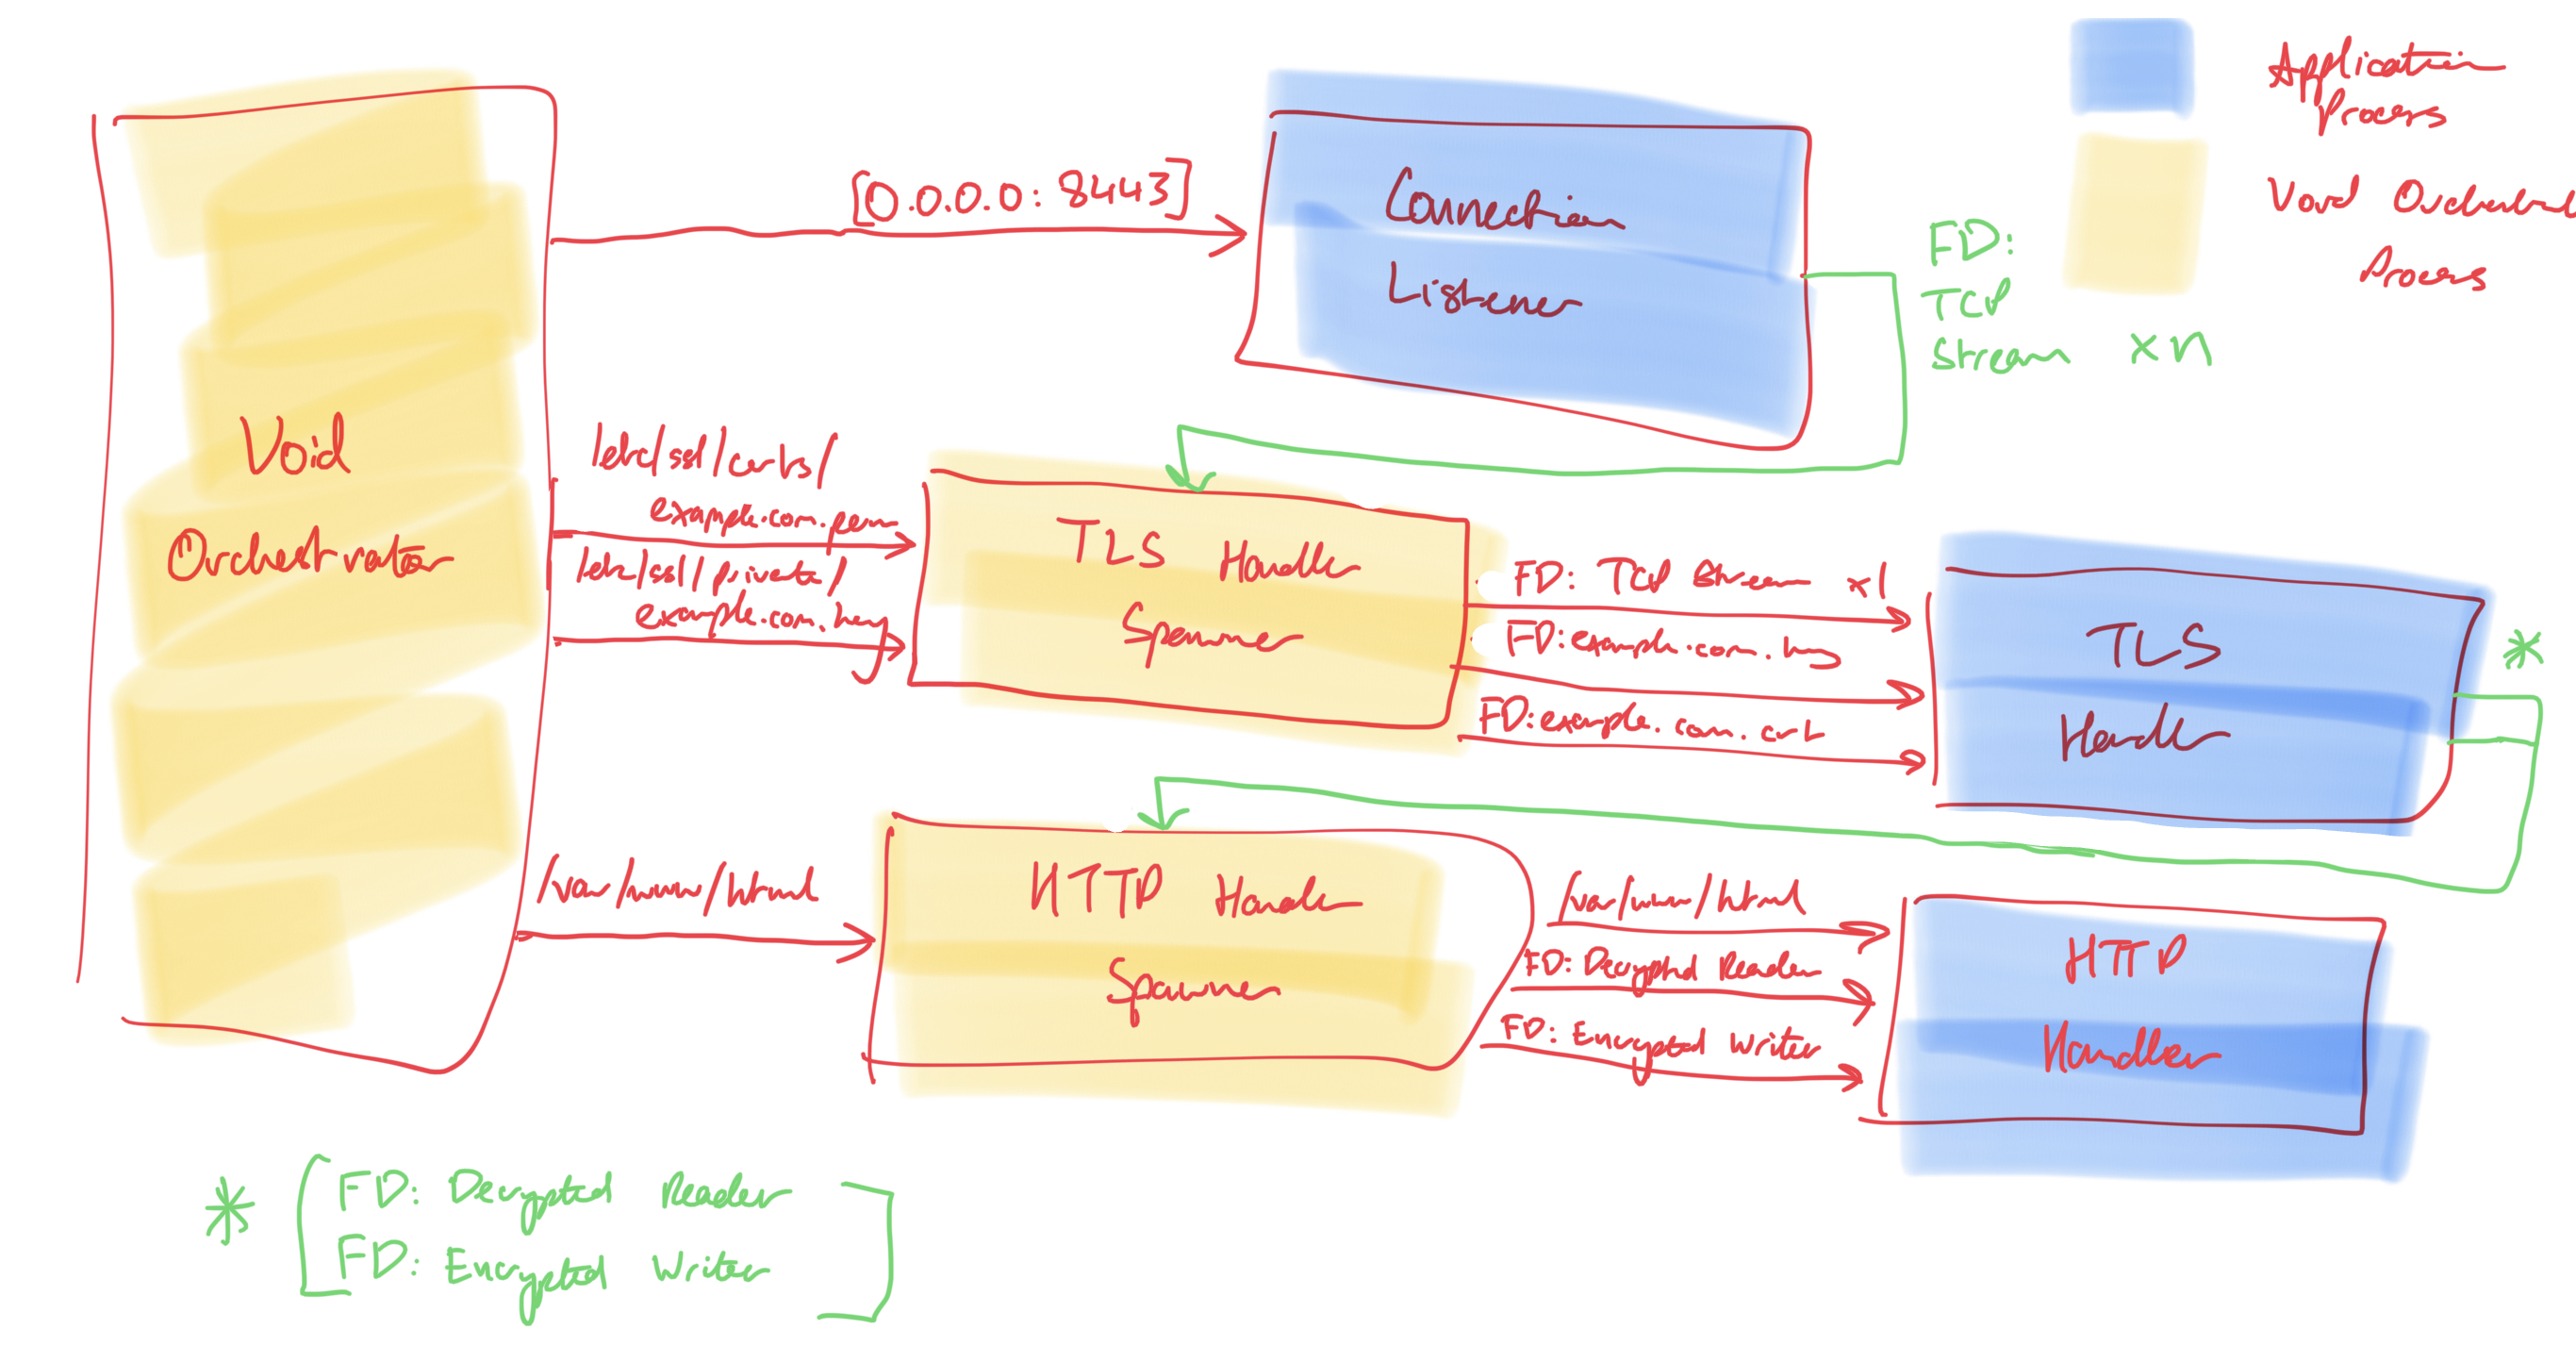
\includegraphics[width=\columnwidth]{figures/tls-server-splitting.png}
    \caption{Process separation in a TLS server.}
    \label{fig:tls-server-splitting}
\end{figure}

Finally, a rudimentary TLS server is created to show the rich privilege separation abilities of multi-entrypoint applications. An example structure is shown in Figure \ref{fig:tls-server-splitting}. Rather than being provided with a view of the network, the initial TCP handling process is given an already bound socket listener by the shim. This allows the TCP handler to live in an extremely restricted zero-access network namespace, while still performing the tasks of receiving new TCP connections.

Next, the TCP handler hands off the new TCP connections to the shim. Though the figure shows this as a direct connection between the TCP handler and the TLS handler, they are passed through the shim, from which the shim spawns a fresh TLS handler for each connection. The TLS handler is handed file descriptors to the certificate and key files that it requires, and hands back a decrypted request reader and an empty response writer file descriptor to the shim.

Finally, this pair of decrypted request reader and response writer are handed to a new process which handles the request. In the example case, this new process is handed a dirfd to \texttt{/var/www/html}, which is bind-mounted into an empty file system namespace by the shim. This allows the request handler enough access to serve files, while restricting access to anything else.


\chapter{Evaluation}
\label{chap:evaluation}

\todo{Write evaluation}

\section{Startup performance}
\label{sec:evaluation-startup-perf}

\todo{Write section on startup performance.}


\chapter{Conclusions}
\label{chap:conclusions}

The system built in this project enables running applications with minimal privilege in a Linux environment in a novel way. Performance is shown to be comparable, and demonstrates where the existing kernel setup provides inadequate performance for such applications. Design choices in the user-space kernel APIs for namespaces are discussed and contextualised, with suggestions offered for alternate designs.

Void Processes offer a new paradigm for application development which prioritises privilege separation above all else. Rather than focusing on limiting backward compatibility, applications often need to be completely rewritten in order to take advantage of improved isolation. The system is designed to support effective static analysis on applications, though this is not implemented at this stage.

Finally, Void Processes provide a seamless experience without making kernel level changes, allowing for ease of deployment. Moreover, it runs on the Linux kernel, a production kernel and not a research kernel. Although the current kernel structure limits the performance of the work with namespace creation being the bottleneck, the feasibility of namespaces for process isolation is effectively demonstrated in a system that encourages application writers to develop with privilege separation as a first principle.

\section{Future Work}

\subsection{Kernel API improvements}

The primary future work to increase the utility of void processes is better performance when creating empty namespaces. Section \ref{sec:evaluation-startup-perf} showed that the startup hit when creating the namespaces for a void is very high. This shows a limitation of the APIs, as creating a namespace that has no relation to a parent should involve a small amount of work. Secondly, an API similar to network namespaces adding paired interfaces between namespaces should be added for binding in mount namespaces, allowing mount namespaces to also be created completely empty. This would also benefit containers which by default have no connection to the parent namespace, but need to mount in their own root filesystem.

\subsection{Dynamic linking}

Dynamic linking works correctly under the shim, however, it currently requires a high level of manual input. Given that the threat model in Section \ref{section:threat-model} specifies trusted binaries, it is feasible to add a pre-spawning phase which appends read-only libraries to the specification for each spawned process automatically before creating appropriate voids. This would allow anything which can link correctly on the host system to link correctly in Void Processes.

\subsection{Dynamic requests}

In Section \ref{sec:filling-net} a system was presented for dynamically requesting statically specified network sockets. This system of requests back to the shim could be extended to more dynamic behaviour for software that requires it. Some software, particularly that which interfaces with the user, is not able to statically specify their requirements before starting. By specifying instead a range of requests which are legal then making them dynamically, Void Processes would be able to support more software.


\appendix
\singlespacing

\bibliographystyle{PhDbiblio-url} 
\bibliography{references} 

\end{document}
